\section{How to add figures and pictures to your thesis}


Here are a few examples of how to add figures or pictures to your thesis (see Figures~\ref{fig:fnCompModel}, \ref{fig:game-based_proofs}, \ref{fig:proveit_screenshot}).

Rule: All the figures, tables and extras in the thesis have to be referred to somewhere in the text.


\begin{figure} [ht] %try to place the figure here (next option top of the page)
\begin{center}
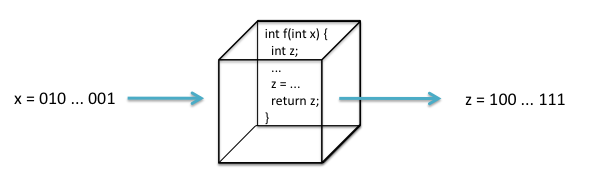
\includegraphics[width=0.8\textwidth]{computational_model_function}
\caption{The title of the Figure.}
\label{fig:fnCompModel}
\end{center}
\end{figure}



\begin{figure} [!ht] %if [h] doesn't work, we can force with !
\begin{center}
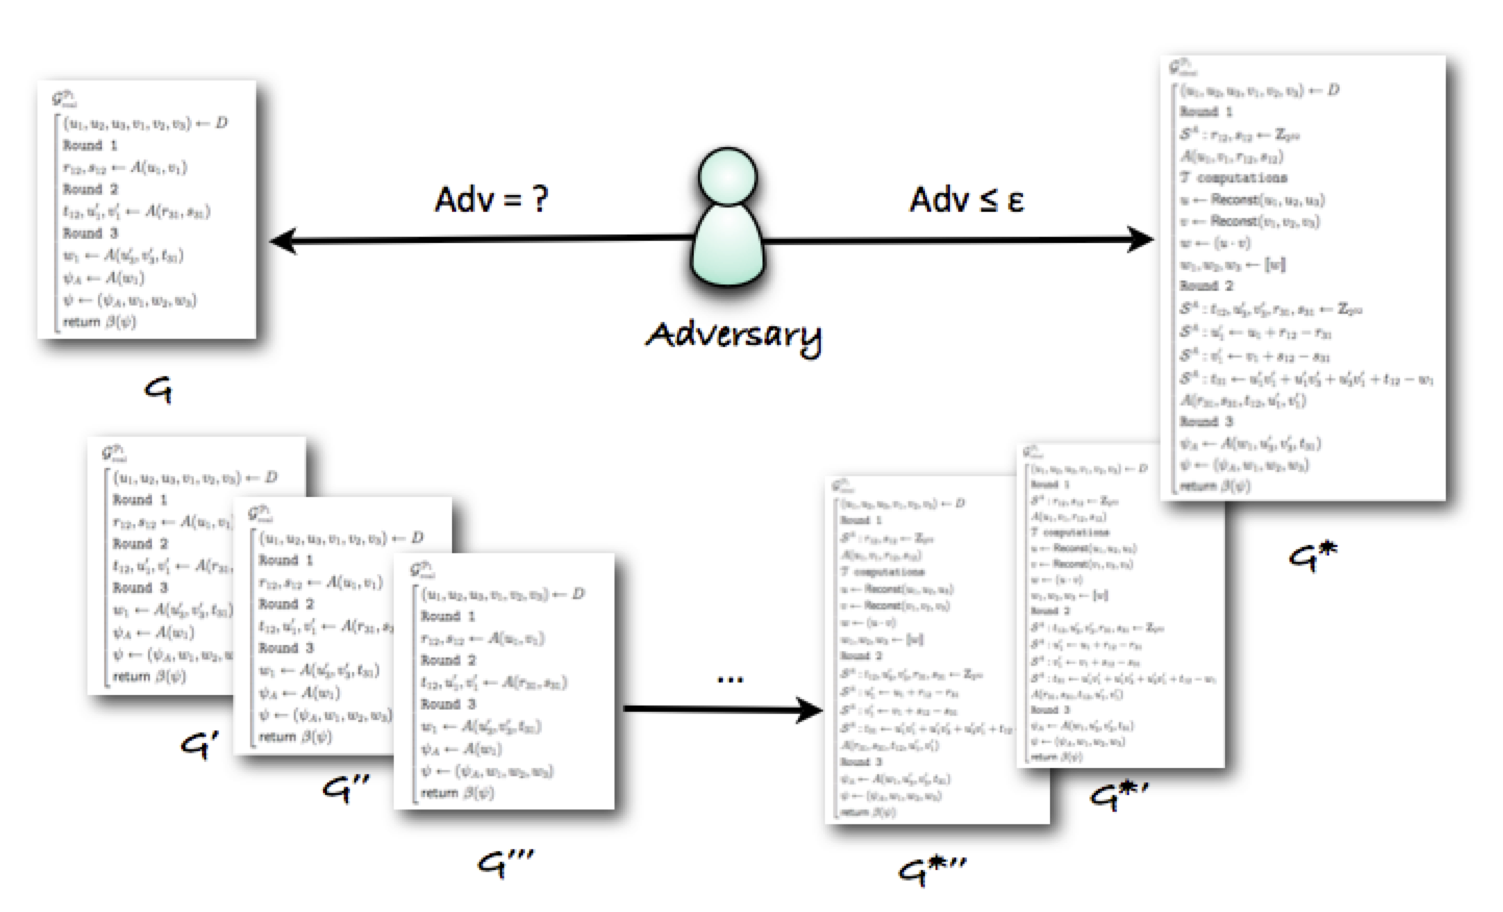
\includegraphics[width=\textwidth]{game-based_proofs}
\caption{Refer if the figure is not yours~\cite{kamm12}.}
\label{fig:game-based_proofs}
\end{center}
\end{figure}


\begin{figure} [p]
\begin{center}
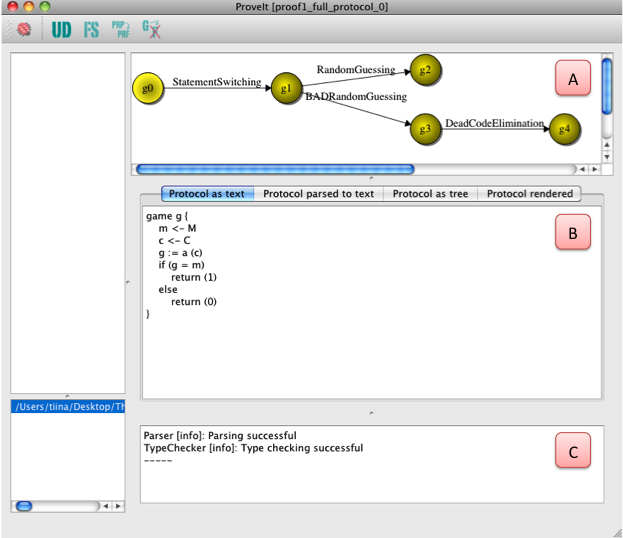
\includegraphics[width=\textwidth]{proveit_screenshot}
\caption{Screenshot of \proveit.}
\label{fig:proveit_screenshot}
\end{center}
\end{figure}

Tip: If you add a screenshot, then labeling the parts might help make the text more understandable (panel C vs bottom left part), e.g.


\begin{figure} [htbp]
\begin{tabular}{c c}
%
\begin{minipage}{0.45\textwidth}
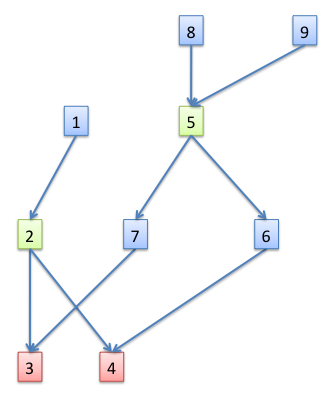
\includegraphics[width=\textwidth]{LCA_2_solutions}
\end{minipage}
%
&
\begin{minipage}{0.55\textwidth}
\centering
\begin{tabular}{cl}
  \toprule
	Node & Decendants \\
  \midrule
  1 & 2, 3, 4 \\
  2 & 3, 4 \\
  3 & \\
  4 & \\
  5 & 3, 4, 6, 7 \\
  6 & 4 \\
  7 & 3 \\
  8 & 3, 4, 5, 6, 7\\
  9 & 3, 4, 5, 6, 7\\
  \bottomrule
\end{tabular}
\end{minipage}
\end{tabular}
%
\caption{Example how to put two figures parallel to each other.}
\label{fig:LCA_2_solutions}
\end{figure}


Example: A screenshot of \proveit can be seen in Figure~\ref{fig:proveit_screenshot}. The user first enters the pseudocode of the initial game in panel B. \proveit also keeps track of all the previous games showing the progress on a graph seen in panel A.

There are two figures side by side in Figure~\ref{fig:LCA_2_solutions}.
